% solving_model_roi_execution_summary.tex
% One-page executive summary + appendix, standard IEEEtran article format.
% Content mirrors solving_model_roi_execution_summary.md verbatim.

\documentclass[10pt,onecolumn]{IEEEtran}

\usepackage{graphicx}
\usepackage{fancyhdr}
\usepackage{xcolor}
\usepackage{booktabs}
\usepackage{float}
\usepackage[colorlinks=true, linkcolor=blue, urlcolor=blue, citecolor=blue]{hyperref}

\definecolor{amdred}{HTML}{00A651}

\title{AMD-Sourcing the Engineering Cycles to Close NVIDIA's Physical-AI Lead: A Challenge/Leaderboard}
\author{Hari Krishna Vydana}

\begin{document}

\maketitle

\pagestyle{fancy}
\fancyhf{}
\cfoot{\thepage}
\renewcommand{\headrulewidth}{0pt}
\thispagestyle{fancy}

\large

AMD hardware already wins on economics --- roughly 50\% lower capex and 30\% lower opex than the incumbent, on competitive silicon (MI300X, Ryzen AI, Kria). Yet application developers still say no, because their products are already built around NVIDIA's models and pipelines (NGC, TensorRT, Isaac ROS, cuRobo, Isaac Sim, Cosmos). NVIDIA's moat is roughly 80\% ecosystem and 20\% hardware: 2M+ robotics developers, a 7+-year head start. Re-hosting a deployment costs 6--18 engineer-months and 5--7 re-targeted artifacts per model --- a bill the customer, not AMD, has to pay before hardware economics even enter the conversation. That burden falls hardest on the small and mid-size robotics companies AMD most needs to win. Internally, this gap is known and winnable but cannot be closed by any single business unit: model training is iterative, the payoff is multi-year, and no BU can book near-term ROI on it --- so, rationally, nobody starts, and the gap widens.

The way out is to pose this as a \textit{replication problem, not an invention problem}. The target models are named, mostly open, and their performance is already published on NGC --- we know exactly what ``done'' looks like. Only two things are missing: compute, which AMD already has (ALOLA and other AMD-wide clusters), and data, the real work (synthetic generation, pooled and curated open data, semi-supervised labeling, pseudo-labels from large open-source models and data pools). The proposal is an AMD-wide model training challenge: pick a target model, train it on AMD compute, submit a per-model leaderboard, and have PAVS validate and publish the result. This pattern has closed comparable capability gaps before --- ImageNet seeded the deep-learning era, the DARPA Grand Challenge seeded self-driving, and Kaggle/Netflix Prize crowdsourced solutions that beat in-house teams at a fraction of the cost. A scored, public target repeatedly does what no single roadmap can.

The mechanism is self-sustaining because every party wins by playing: participating engineers get recognition, a publishable track record, and a countable contribution to AMD; PAVS becomes the customer gateway for physical AI and the bridge across AMD's distributed teams; and AMD closes a strategic ecosystem gap with pooled compute and no single-BU budget line, building a pipeline of market-ready, AMD-native models and datasets along the way. The prize is worth the effort --- AMD projects a \$200B physical-AI silicon market by 2035, robotics startup funding hit \$22.2B in 2025 (+69\% YoY). Of 125 NGC models scanned, 48 across four priority tiers need an AMD-native replica (Appendix, Tables~\ref{tab:a1}--\ref{tab:a4}); Tier 1 + Tier 2 (30 models) is the actual ``customer has this running on NVIDIA today and can't move it'' set.

\normalsize
\newpage
\begin{center}
{\huge\bfseries\color{amdred}The Ask}
\end{center}
\vspace{0.5em}
\textit{The plan is already staffed --- we only need the mandate to start.}

\textbf{What we need from leadership:} an org-wide email endorsing the challenge --- the signal that gives the effort good traction.

\begin{figure}[H]
\centering
\begin{minipage}{0.5\linewidth}
\centering
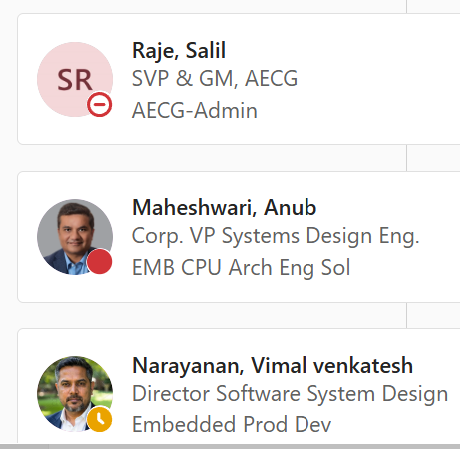
\includegraphics[width=0.8\linewidth]{../contibutors/Upperlevel_management.png}\\[3pt]
{\small Leadership endorsement}
\end{minipage}

\vspace{0.7em}

\begin{minipage}{0.4\linewidth}
\centering

\includegraphics[width=0.8\linewidth]{../contibutors/mathew.png}\\[3pt]
{\small Compute (ALOLA)}
\end{minipage}\hfill
\begin{minipage}{0.4\linewidth}
\centering

\includegraphics[width=0.8\linewidth]{../contibutors/Bharat.png}\\[3pt]
{\small Per-model GitHub}
\end{minipage}

\vspace{0.1em}

\begin{minipage}{0.62\linewidth}
\centering
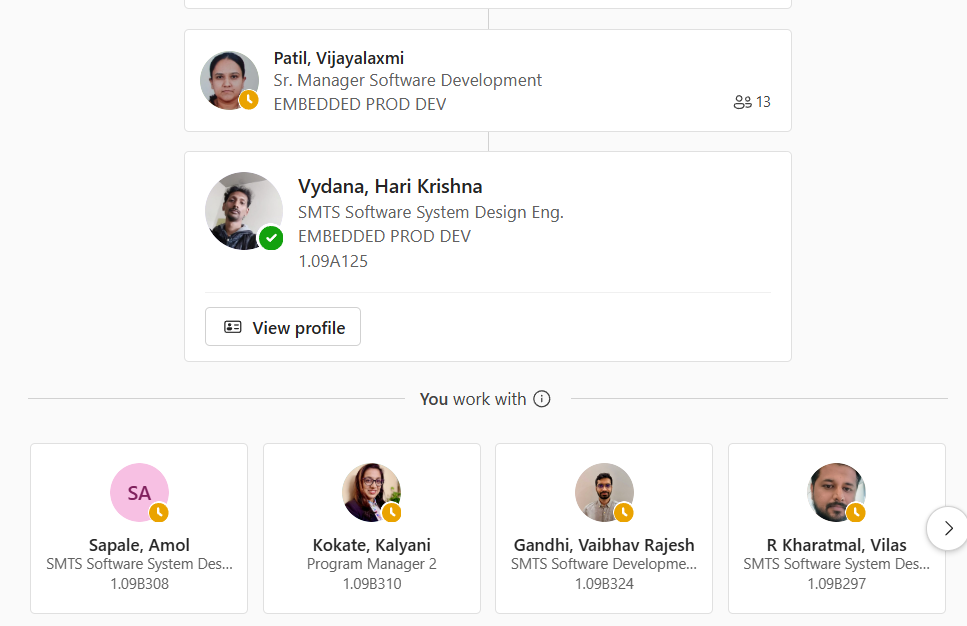
\includegraphics[width=\linewidth]{../contibutors/Team_participation.png}\\[3pt]
{\small Team to execute}
\end{minipage}

%\vspace{0.2em}
\caption{Already staffed and committed: leadership signal, compute, repos, and team are all in place --- all that's missing is the go-ahead.}
\label{fig:ask}
\end{figure}

\newpage
\appendices
\section{NGC Physical-AI Target Set}

\begin{table}[H]
\centering
\caption{Tier 1 --- Production Perception Stack (NVIDIA Metropolis/DeepStream). Highest priority --- most commonly deployed NGC models a customer runs today and cannot carry over to AMD.}
\label{tab:a1}
\footnotesize
\begin{tabular}{@{}p{1.6in}p{2.1in}p{2.3in}@{}}
\toprule
NVIDIA model & Function & Why it matters \\
\midrule
TrafficCamNet & Vehicle detection (traffic cameras) & Core Metropolis/smart-city SKU \\
PeopleNet / PeopleNet-AMR & Person detection & Most widely deployed DeepStream model \\
LPRNet + LPDNet & Plate detection + recognition pair & Sold as a pair, tolling/parking/security \\
VehicleMakeNet / VehicleTypeNet & Vehicle attribute classification & Paired with TrafficCamNet in the same pipelines \\
ReIdentificationNet (+ Transformer) & Person re-identification across cameras & Retail/security analytics \\
PeopleSemSegNet / AMR & Person segmentation & Privacy-masking, robotics safety zones \\
Retail Object Detection / Recognition & Shelf/product detection & Retail analytics vertical \\
Action Recognition Net & Action/behavior classification & Security, workplace safety \\
BodyPoseNet / PoseClassificationNet & Human pose estimation & Robotics, ergonomics, fitness \\
OCDNet / OCRNet & Scene text OCR & Logistics, document/label reading \\
\bottomrule
\end{tabular}
\end{table}

\begin{table}[H]
\centering
\caption{Tier 2 --- Robotics/Perception Building Blocks (Physical AI). The models Isaac ROS perception pipelines are built on --- closest to AMD-ROS/AARTS. Tier 1 + Tier 2 = 30 models, the real ``customer has this running and can't move it'' set.}
\label{tab:a2}
\footnotesize
\begin{tabular}{@{}p{2.2in}p{4.0in}@{}}
\toprule
NVIDIA model & Function \\
\midrule
Bi3D Proximity Segmentation & Stereo-based obstacle proximity \\
ESS DNN Stereo Disparity & Stereo depth \\
FoundationPose & 6-DoF object pose estimation/tracking \\
PointPillarNet & LiDAR 3D object detection \\
Transfusion (3D Object Detection) & Camera+LiDAR fusion detection \\
CitySemSegFormer & Semantic segmentation (autonomy/city-scale) \\
TAO Pretrained (Classification/DetectNet V2/EfficientDet/Instance Seg/Semantic Seg) & Generic backbones customers fine-tune on top of --- AMD needs some pretrained backbone family here or customers cannot start a TAO-style workflow on AMD \\
\bottomrule
\end{tabular}
\end{table}

\begin{table}[H]
\centering
\caption{Tier 3 --- Biometric/Human-Sensing (smaller but sticky niche). Matters mainly if AMD is also chasing the biometric/kiosk vertical.}
\label{tab:a3}
\footnotesize
\begin{tabular}{@{}p{2.2in}p{4.0in}@{}}
\toprule
NVIDIA model & Function \\
\midrule
FaceNet & Face detection \\
FaceDetectIR & Face detection (infrared) \\
GazeNet & Gaze tracking \\
EmotionNet & Emotion classification \\
GestureNet & Hand/body gesture recognition \\
HeartRateNet & Remote heart-rate estimation \\
Facial Landmark Estimator (FPENet) & Facial landmark detection \\
Deformable DETR (NvImageNet weights) & Detection backbone \\
FAN (NVImageNet weights) & Classification backbone \\
GCViT (NVImageNet weights) & Classification backbone \\
Visual ChangeNet Classification & Change detection classification \\
NVIDIA Optical Inspection Model & Industrial visual inspection \\
\bottomrule
\end{tabular}
\end{table}

\begin{table}[H]
\centering
\caption{Tier 4 --- Enterprise Vision \& HPC/Climate (lowest priority). Matters mainly if AMD is also chasing the enterprise-vision or HPC-climate vertical.}
\label{tab:a4}
\footnotesize
\begin{tabular}{@{}p{1.6in}p{2.1in}p{2.3in}@{}}
\toprule
NVIDIA model & Function & Why lower priority \\
\midrule
PCB Defect Classification & Industrial inspection & NVIDIA AI Enterprise EULA; small footprint \\
PeopleSemSegFormer & Person segmentation & NVIDIA AI Enterprise EULA; small footprint \\
DINO (NvImageNet weights) & Classification backbone & NVIDIA AI Enterprise EULA; small footprint \\
PhysicsNeMo: AFNO\_DX\_FI-V1-ERA5 & Weather forecasting & Community Model License; HPC/climate-only \\
PhysicsNeMo: AFNO\_DX\_SR-V1-ERA5 & Weather forecasting & Community Model License; HPC/climate-only \\
PhysicsNeMo: AFNO\_DX\_TP-V1-ERA5 & Weather forecasting & Community Model License; HPC/climate-only \\
PhysicsNeMo: AFNO\_DX\_WG-V1-ERA5 & Weather forecasting & Community Model License; HPC/climate-only \\
PhysicsNeMo: DLESyM-V1-ERA5 & Weather forecasting & Community Model License; HPC/climate-only \\
\bottomrule
\end{tabular}
\end{table}

48 models across four tiers, out of 125 scanned on NGC --- the other 77 are either already portable (49) or unresolved catalog entries (28).

\end{document}
